\documentclass[10pt,a4paper,twocolumn]{article}
\usepackage[a4paper, margin=0.7in]{geometry}
\usepackage[utf8]{inputenc}
\usepackage{amsmath}
\usepackage{amsfonts}
\usepackage{amssymb}
\usepackage{graphicx}
\usepackage{subcaption}
\usepackage[numbers,sort]{natbib}
% === FOR TABLE ===

\usepackage[usenames,dvipsnames]{xcolor}
\usepackage{tcolorbox}
\usepackage{tabularx}
\usepackage{array}
\usepackage{colortbl}
\tcbuselibrary{skins}
\newcolumntype{Y}{>{\raggedleft\arraybackslash}X}

\tcbset{tab1/.style={fonttitle=\bfseries\large,fontupper=\normalsize\sffamily,
colback=yellow!10!white,colframe=red!75!black,colbacktitle=Salmon!40!white,
coltitle=black,center title,freelance,frame code={
\foreach \n in {north east,north west,south east,south west}
{\path [fill=red!75!black] (interior.\n) circle (3mm); };},}}

\tcbset{tab2/.style={enhanced,fonttitle=\bfseries,fontupper=\normalsize\sffamily,
colback=yellow!10!white,colframe=red!50!black,colbacktitle=Salmon!40!white,
coltitle=black,center title}}
% === END TABLE ===

\makeatletter
\renewcommand{\maketitle}{\bgroup\setlength{\parindent}{0pt}
\begin{flushleft}
  \textbf{\LARGE \@title}
  
  \@author
\end{flushleft}\egroup
}
\makeatother


\author{%
\textbf{\large Ahmet Emre Aladağ$^{1}$}\\
$^{1}$Boğaziçi Üniversitesi, Bilgisayar Mühendisliği Bölümü, İstanbul\\
	emre.aladag@boun.edu.tr
}

\title{İstanbul Toplu Taşıma Ağı Analizi}
\newcommand{\buyukkalin}[1]{\Large\textbf{#1}}
\renewcommand{\figurename}{Şekil}
\renewcommand{\tablename}{Tablo}
\renewcommand\refname{Kaynaklar}
\providecommand{\anahtar}[1]{\textbf{Anahtar Kelimeler:} #1}
\providecommand{\ozet}[1]{\textbf{Özet:} #1}
\providecommand{\keywords}[1]{\textbf{Keywords:} #1}
\providecommand{\abstractt}[1]{\textbf{Abstract:} #1}
\providecommand{\englishtitle}[1]{\buyukkalin{#1}}

%\providecommand{\keywords}[1]{\textbf{\textbf{Anahtar Kelimeler:}} #1}


\begin{document}

\twocolumn[
  \begin{@twocolumnfalse}
    \maketitle
	\begin{ozet}
	Trafik sıkışıklığı, günümüz metropollerinin en büyük sorunlarından birisidir. Dünyada her gün milyonlarca saat trafik sebebiyle boşa gitmekte, çalışanların ve öğrencilerin verimi düşmektedir. Trafiği azaltmak için trafiğe katkıda bulunan etkenlerin tespit edilip çözüm yoluna gidilmesi elzemdir. Çözüme yönelmeden önce sorunun asıl kaynağı iyice tespit edilmelidir. Hatalı tasarlanan ulaşım altyapıları yahut plansız kentleşme bu kaynakların en önemlilerindendir. Bu çalışma, İstanbul'daki toplu taşıma ağının analiz edilerek şehirdeki yapısal darboğazların tespit edilmesini amaçlamaktadır. Otobüs güzergahlarının konumsal ağ şeklinde kurgulanıp analiz edilmesiyle trafik yoğunluğunun oluşabileceği noktalar tespit edilmiştir ve tespitler gerçek hayat deneyimleriyle uyumludur.
	\end{ozet}
	\newline
	\newline
    \begin{anahtar}
    veri görselleştirme, ağ bilimi, çizge, toplu taşıma, ulaşım ağı
    \end{anahtar}
	\newline
	\newline
	\begin{englishtitle}
		\bf Istanbul Public Transportation Network Analysis
	\end{englishtitle}
	\newline
	\newline	
    \begin{abstractt}
	Traffic congestion is one of the major problems of metropolitan cities. Each day millions of hours are wasted due to traffic congestion in the world, causing reduction in productivity among workers and students. In order to reduce traffic congestion, it is required to figure out major factors contributing to the congestion. The faults in the design of the transportation infrastructures or unplanned urbanization are some among the most important factors. This study aims to detect bottlenecks in the transportation network of Istanbul via network analysis. We detected potential traffic congestion points using bus line route information represented as a spatial transportation network. Our detections are complying with our real life experience.
    \end{abstractt}
	\newline
	\newline
    \begin{keywords}
	visualization, network science, spatial graph, transportation network
    \end{keywords}
	\newline
	\newline
  \end{@twocolumnfalse}
]

\section{Giriş}
\paragraph{} Son yıllarda şehirleşmenin ve araç sayısının artmasıyla birlikte büyük şehirlerde trafik sıkışıklığı sorunu başgöstermiştir. Trafik sıkışıklığının en önemli sebepleri arasında plansız kentleşme ve kontrolsüz göç yer almaktadır. Her geçen gün artan ve 2016 itibariyle 14 milyonu geçen nüfusuyla İstanbul, trafik sıkışıklığının en yoğun olarak görüldüğü dünya şehirlerinden biridir. Bu çalışmadaki araştırma sorumuz \textit{"Otobüs güzergahlarını inceleyerek İstanbul şehrindeki yapısal darboğazları (trafiğin sıkıştığı noktaları) tespit edebilir miyiz?"} olacaktır. Analizlerimiz ağ tabanlı yapısal bir analizin gerçekte trafik yoğunluğu yaşanan noktaları tespit edebilmekte olduğunu göstermektedir. Çalışmamız için gerekli verileri İstanbul Büyükşehir Belediyesi'nin sunduğu \textit{Açık Veri} platformu olan \textit{CitySDK} sağlamaktadır. 

\section{Literatür Araştırması}
Ulaşım ağ analizi konusundaki çalışmalar \cite{lam1982connectivity,bell1997transportation} çok eskiye dayansa da ağ biliminin ve simülasyon altyapılarının gelişmesi ve veri miktarının artmasıyla birlikte son yıllarda canlanmış, ağ temelli yapısal analizler, ulaşım altyapı planlamaları, tarife tablolarının belirlenmesi, trafiğin modellenmesi gibi çalışmalar görülmüştür.

Soh ve ekibi Singapur tren taşıma ağının ve şehirleşme yapısının analizini yapmıştır \cite{soh2010weighted} ancak hedefinde trafik sıkışıklığı yoktur. Derrible ve ark. metro ağlarının dayanıklılığını \cite{derrible2010complexity} incelemiştir. Lam ve ark. ise en verimli transit sistemini kurma amaçlı çalışmalar \cite{lam1982connectivity} yürütmüştür.

Toplu taşıma sistemlerinin çoklu ajan modellemesini yapan ve olası sorunları simüle etmeye yönelik çalışmalar da \cite{balbo2001toward,von2007network,von2009public,levinson2006self} mevcuttur. Toplu taşıma sistemlerinde sorun yaşanabilecek zayıf noktaları tespit etmeye yönelik başlıca çalışmalar Scott ve ark.  tarafından yürütülmüştür \cite{scott2006network}. Şehirlerin büyümesiyle birlikte ulaşım ağlarının gelişimini inceleyen \cite{xie2009modeling}, trafik akışını, ulaşım planlamasını ve ağ gelişiminin ekonomisini ele almıştır. Trafik konusuna eğilen \cite{sun2008dynamics}, yol genişliği, araç hızı gibi mikroskopik özellikleri kullanarak bir akış modeli üzerinden trafik dinamiklerini incelemiştir. LeBlanc ve ark. çalışmasında trafik akışının dengelenmesi üzerine çalışmalar \cite{leblanc1975efficient} yürütmüştür. 

Pattnaik ve ark. genetik algoritma kullanarak transit güzergah tasarımı üzerinde çalışmalar \cite{pattnaik1998urban} yürütürken, Baaj ve ark. transit ağ tasarımında buluşsal algoritmaların kullanımını \cite{baaj1995hybrid} önermiştir. Bununla birlikte Jian ve ark. en az sayıda duraksama yaparak en ekonomik seyahat edilebilecek bir ulaşım sistemi tasarlayan algoritma \cite{jian2005public} geliştirmiştir. Goczylla ve ark. bir ulaşım ağında en optimal güzergahın tespitine yönelik buluşsal bir algoritma \cite{goczylla1995optimal} geliştirmiştir.  Mandl ve ark. de toplu taşıma sistemlerinin eniyileştirilmesi ve değerlendirilmesine yönelik çalışmalarda \cite{mandl1980evaluation} bulunmuştur. Sheffil ve ark. ise, olası bir afet durumunda şehrin boşaltılmasının en kısa ve güvenli sürede yapılabilmesi için bir çerçeve \cite{sheffi1982transportation} çizmiştir. Bununla birlikte İstanbul büyüklüğünde bir şehrin otobüs altyapısını ağ bazlı inceleyerek olası darboğazları tespit edecek uygulamaya yönelik bir çalışma bildiğimiz kadarıyla yoktur.

\section{Yöntem}
\subsection{Veri Kaynağı}
\paragraph{} Bu çalışmada veri kaynağı olarak kullandığımız CitySDK, toplu taşıma sistemlerine dair açık veri sunulmasını amaçlayan AB tarafından desteklenen bir projedir. Proje, dünya çapında 8 şehirde denenmiştir, bunlardan birisi de İstanbul'dur. İstanbul Büyükşehir Belediyesi, toplu taşıma bilgilerine ücretsiz erişim sağlayan bir API sunmaktadır. Bu API, İstanbul'daki otobüs hatlarının listesini ve bu hatların sırayla hangi duraklardan geçtiğini koordinatlarıyla birlikte sorgulama imkanı sunmaktadır. Biz de \textit{Python} programlama dili ile yazılmış olan \textit{Scrapy} sürüngen kütüphanesi ile hat listesini ve her güzergahta yer alan durakları koordinatlarıyla çektik. Elde ettiğimiz verileri de \textit{R programlama dili} ve \textit{igraph, ggmap} gibi kütüphanelerini kullanarak işleyip görselleştirdik. Görselleştirdiğimiz veriler 07.07.2015 tarihindeki güzergah bilgilerini baz almaktadır.

\subsection{Veri Yapıları}

\paragraph{} API'dan aldığımız veriler genel olarak liste veri yapısındadır: hat listesi ve bir otobüsün takip ettiği güzergahtaki durakların listesi. İkinci listedeki her bir öğe, güzergah durakları sıralı verildiği için, ardışık olduğu öğelerle ilişkilidir. Biz de bu ilişkiyi kullanarak bir ağ (network/graph) oluşturduk. Bu ağda düğümleri otobüs durakları, kenarları ise iki durak arasındaki güzergah varlığı olarak tanımladık. Örneğin 59R hattı önce \textit{Nispetiye}, sonra \textit{Boğaziçi Üniversite} duraklarından (düğümlerinden) geçiyorsa $u=Nispetiye, v=Bogazici Universite$ olmak üzere iki düğüm arasında yönlü $e = (u, v)$ kenarı oluşturup \textit{59R} hat koduyla etiketledik.

\paragraph{} Ağı görselleştirirken her bir düğüme API'dan elde ettiğimiz koordinatları görsel koordinat olarak atadık. Bu sayede düğüm konumları sabit kalırken kenarlar düğümler arasında görselleşmiş oldu. Bu görselleştirmede bir varsayımımız veri yetersizliği sebebiyle otobüslerin iki durak arasında kuş uçuşu doğrusal olarak gittikleri varsayımı oldu. İleriki çalışmalarda coğrafi veri sistemlerinden alınacak yol koordinatları ile (kenar ara noktaları olarak belirlenerek) çok daha doğru ve yumuşak geçişli görseller elde edilebilir.

\section{Analiz}
\subsection{Çoklu Çizge}
\paragraph{} Öncelikle oluşturduğumuz yönlü ağı çoklu çizge (multigraph) şeklinde görselleştirdik. Bu çizge türünde iki düğüm arasında birden fazla kenar olabilmektedir. Bu durum kenarların üst üste binmesine sebep oldu ama yine de büyük resmi görme açısından Şekil \ref{fig:multigraph} gibi açıklayıcı bir görsel üretti. Görselde düğümler siyah noktalarla temsil ediliyorken kenarlar sarı renkle temsil edildi. Ana arterlerde üst üste binen kenarlar sebebiyle kalınlaşmalar ve doğrusal kenar varsayımımız sebebiyle birtakım kestirme kenarlar görülebilmektedir.

\subsection{Ağırlıklı Ulaşım Ağı}
\paragraph{} Şekil \ref{fig:multigraph}'daki gibi bir veri yapısı ve görselleştirmesinde çok sayıda kenarın üst üste binmesi sebebiyle çok değerli bir bilgiyi kaybediyorduk: iki düğüm arasındaki kenar sayısı. Bu sebeple iki düğüm arasından geçen $x$ adet kenarı, ağırlığı $w(u,v) = x$ olan tek bir $e=(u,v)$ kenarına dönüştürdük. Bu sayede çoklu çizgeyi (Multigraph), tekil çizgeye (Regular graph) çevirmiş olduk. Ardından Şekil \ref{fig:weightedgraph} görselinde kenar ağırlıklarını renk tonu ile temsil ettik: koyu kenarlar en çok hattın geçtiği, en yoğun kenarları temsil etmektedir.

\subsection{Kenar Arasındalığı Analizi}
\paragraph{} İki durak arasından geçen hat sayısı trafik hacmini tahmin etmede güzel bir ölçüt olabilir. Bununla birlikte darboğazların daha iyi görülebilmesi için daha farklı ölçütleri kullanmamız gereklidir. Bunlardan başlıcası tüm ağda ikili her düğüm arasında en kısa rotalar hesaplandığında belirli bir kenar üzerinden geçen en kısa rota sayısını temsil eden Kenar Arasındalığı (Edge Betweenness) ölçütüdür.

\paragraph{} Ağımızdaki her kenar için kenar arasındalığı değerlerini hesaplayıp çok ıraksak değerler ürettiği için değerlerin logaritmasını aldık. Ardından kenar kalabalığını gidermek, sadece en yüksek değere sahip kenarları görselleştirmek için $log(ka(e)) < 3$ olan her $e$ kenarını ağımızdan silerek sadece $[3,5]$ aralığındaki log kenar arasındalığına sahip olan kenarları görselleştirdik. Şekil \ref{fig:edgebetweenness}'e baktığımızda İstanbul'un en büyük darboğazları olan \textit{Boğaziçi, Fatih Sultan Mehmet ve Haliç köprüleri, E-5, üç köprüyü birbirine bağlayan yollar (Haliç-Zincirlikuyu, Zincirlikuyu-Levent), Kozyatağı-Kavacık bağlantısı} görülebilmektedir. Bu güzergahlar üzerinde yaşanabilecek trafik kazaları trafiği felç noktasında getirebilmektedir. Sadece otobüs rotalarına bakarak oluşturduğumuz görselleştirmemizin sonucu bireysel tecrübelerimizle uyuşmaktadır. Bu da İstanbul'daki trafik sorununun altında yatan en önemli etkenlerden birisinin ulaşım altyapısı olduğuna işaret etmektedir.

\subsection{Düğüm Arasındalığı Analizi}
\paragraph{} Bir sonraki aşamada farklı bir açıdan bakıp ağdaki en kısa rotaların hangi düğümlerden geçmek zorunda olduğunu baz alan Düğüm Arasındalığı (Node Betweenness) değerlerini hesapladık. 

\paragraph{} Bu değerleri dikkate alarak bir görselleştirme yaptığımızda farklı darboğazlarla karşılaştık. Şekil \ref{fig:node-betweenness}'de görülebileceği üzere ana arterlerden ziyade sahil yolu gibi trafiğe girildiğinde çıkmanın zor olduğu, alternatif istikametin olmadığı konumları keşfettik. Düğüm Arasındalığı en yüksek olan düğümleri listelediğimizde dikkatimizi çeken duraklardan bazıları şunlardır: \textit{Sabiha Gökçen Havalimanı, Kavacık Köprüsü, Taksim, Eminönü İskele, Yenikapı Sahil, Kumkapı, Sarayburnu, Dolmabahçe Sarayı, 4. Levent}

\section{Sonuç ve Öneriler}
\paragraph{} Sadece otobüs güzergahlarını kullanarak gerçekleştirdiğimiz bu analizle İstanbul'daki potansiyel trafik sıkışıklıklarının hangi noktalarda olabileceğini gösterdik. Potansiyel trafik sıkışıklıklarının bu tür ağ analizi yöntemleriyle tespit edilmesi sayesinde sıkışıklığın ulaşım altyapısının yapısal özelliklerinden kaynaklanıp kaynaklanmadığı görülebilir. Analizimiz trafik etkenlerinden birisinin de İstanbul'da yapısal sorunlar olduğunu işaret etmektedir. Bu tür analizlerin artması için \textit{Açık Veri} sistemleri çok büyük önem arzetmektedir ve yaygınlaşması desteklenmelidir.

\paragraph{} Bu metodoloji, trafik sıkışıklığının üstesinden gelebilmek için hangi noktalara yeni yollar yapılması ve hangi güzergahlarda yeni hatlar açılmasının makul olabileceği konusunda fikir vermektedir. Çalışmanın bölgesel nüfus yoğunluğu verileriyle entegre olması ve sistemin akış (flow) şeklinde modellenmesi doğruluk oranını çok daha artıracaktır. Çalışmamızda kullandığımız kaynak kodlara https://github.com/aladagemre/istanbul-transportation-network adresinden erişilebilir.

\section*{Teşekkürler}
\paragraph{} Bu çalışma Türkiye Bilimsel ve Teknolojik Araştırma Kurulu (TÜBİTAK) tarafından BİDEB 2211-A Programı ile desteklenmiştir.

\bibliographystyle{plain}
%\bibliographystyle{unsrt}
\bibliography{ab16-174} 


\clearpage
\onecolumn
\begin{figure}
\begin{subfigure}{.5\textwidth}
  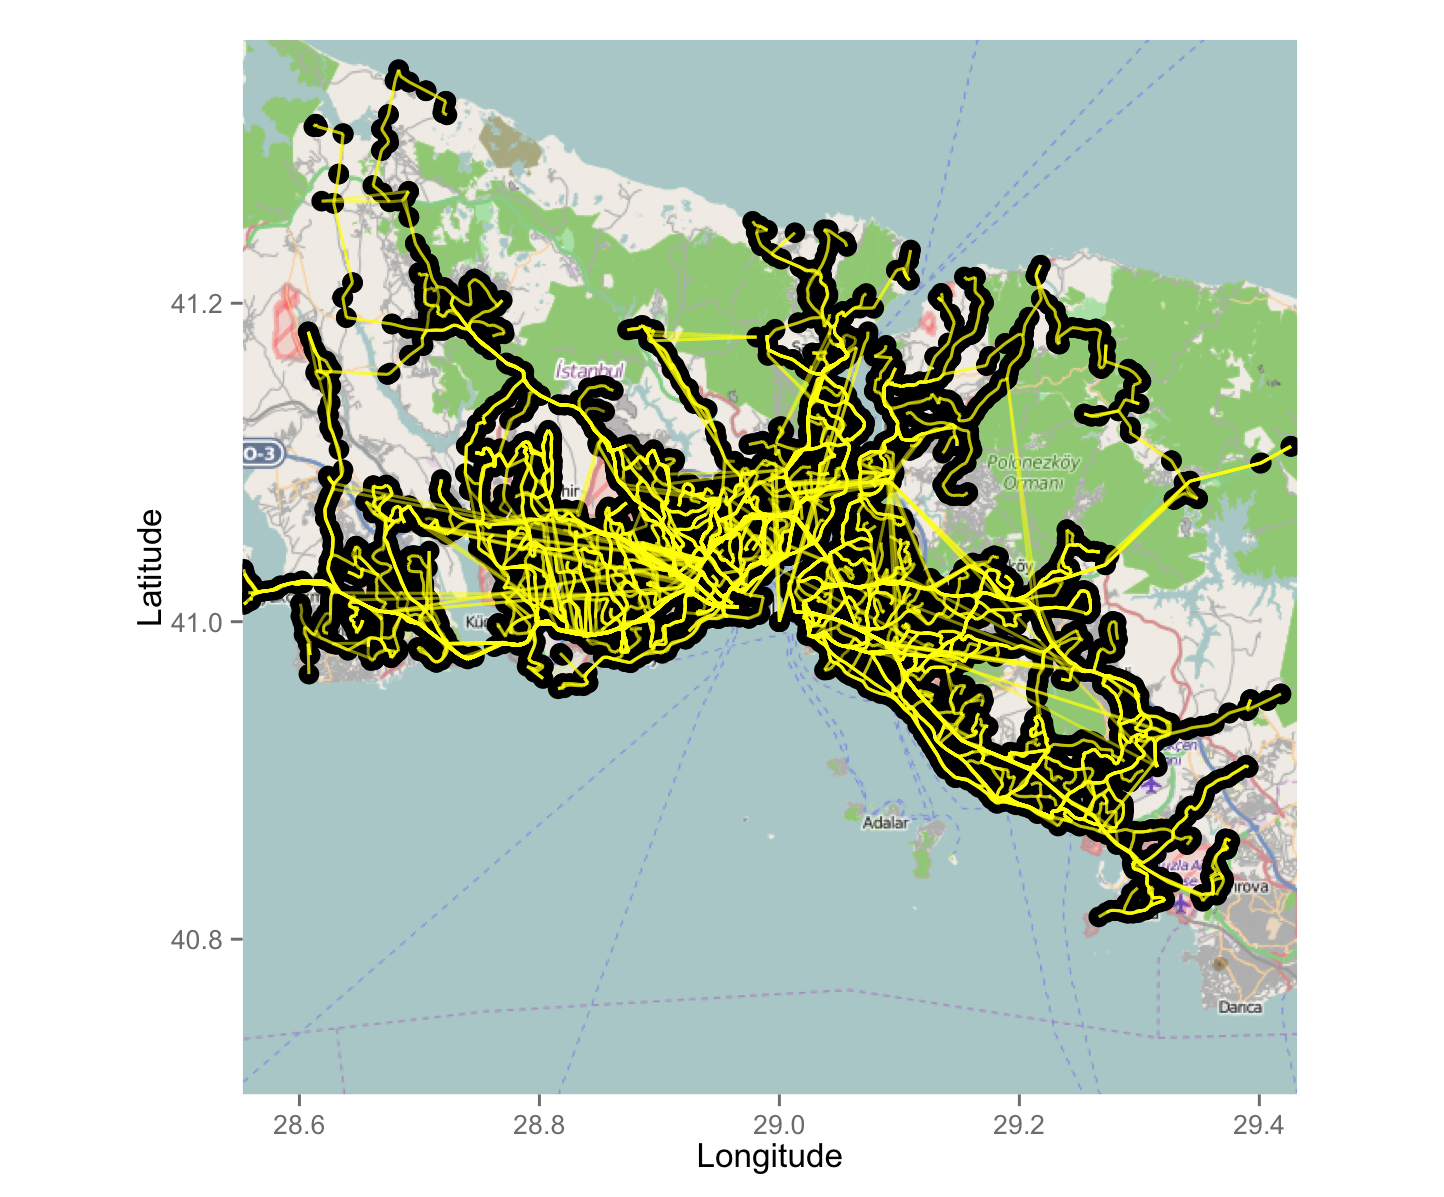
\includegraphics[width=\linewidth]{img/map1-multigraph.png}
  \caption{\textbf{Çoklu Çizge:} Otobüs güzergahlarının çoklu çizge halinde görselleştirilmesi. }
  \label{fig:multigraph}  
\end{subfigure}
\begin{subfigure}{.45\textwidth}
 \hspace{0.1mm}
  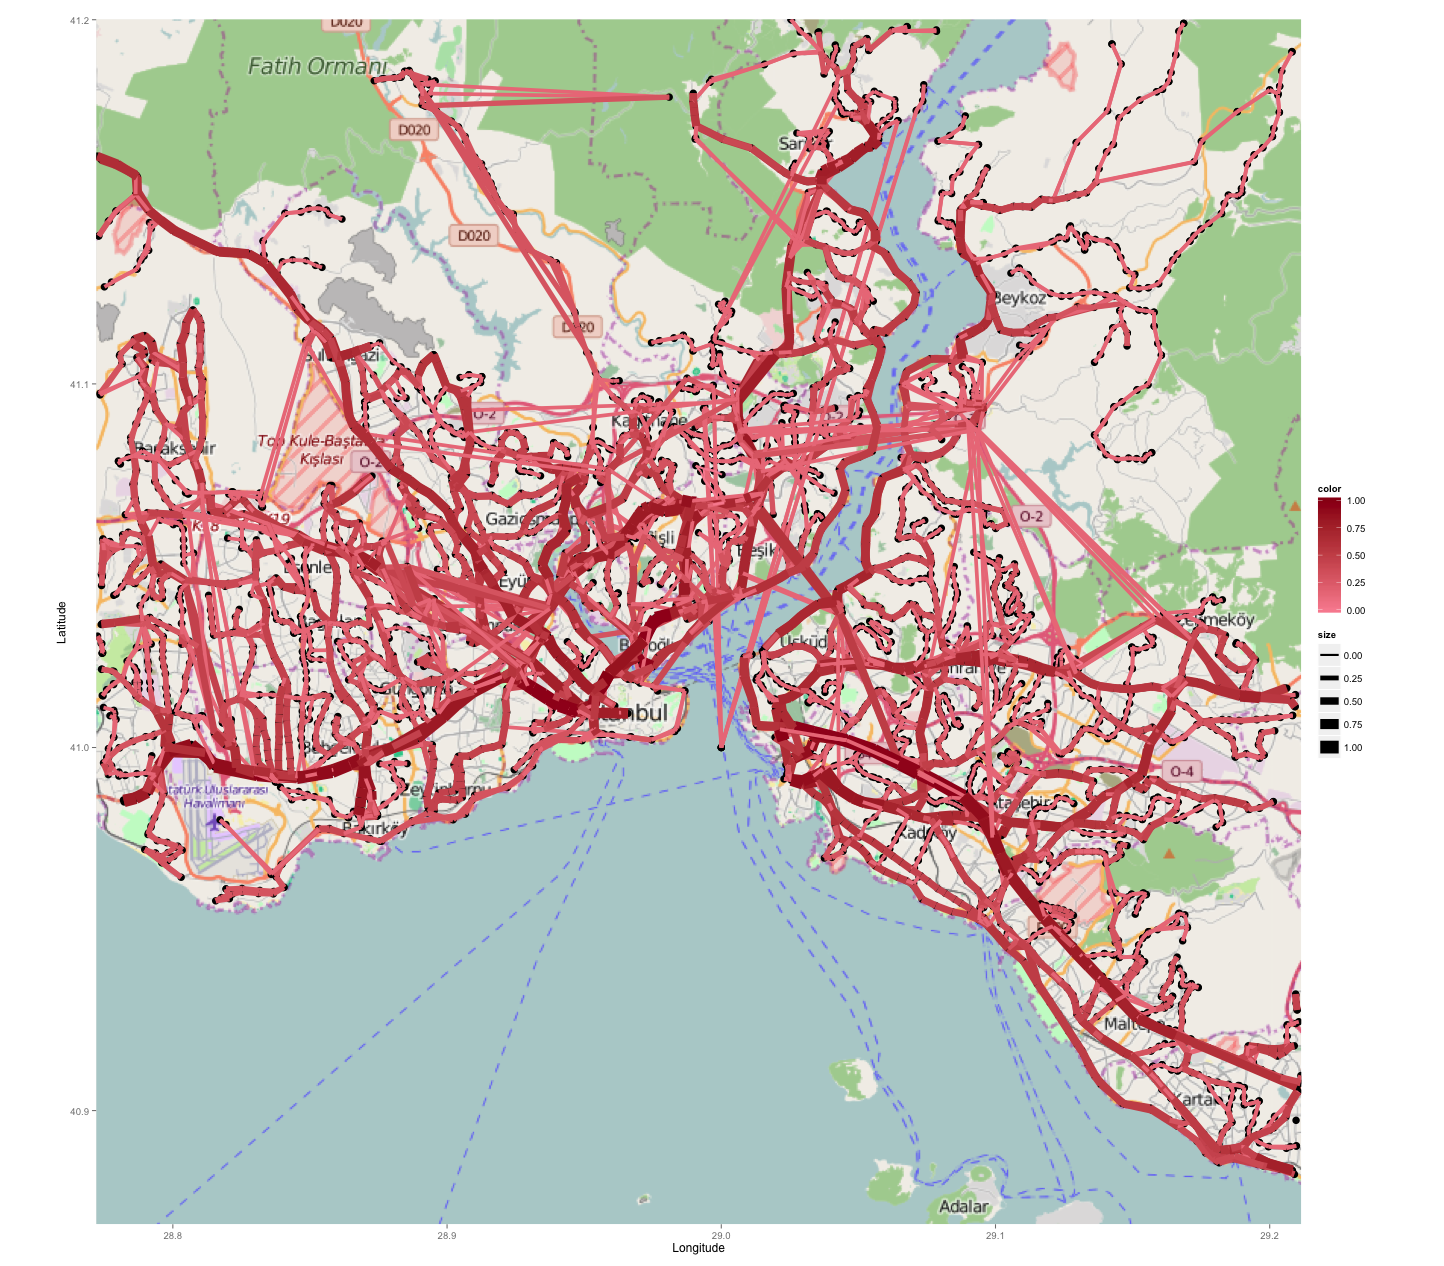
\includegraphics[width=\linewidth]{img/map2-weighted-network.png}
  \caption{\textbf{Ağırıklı Ulaşım Ağı:} aynı kenardan geçen hatların birleştirilmesi ile oluşan ağırlıklı ağ. Koyu renkli ve kalın kenarlardan daha fazla hat geçmektedir.}
  \label{fig:weightedgraph}
\end{subfigure}
\begin{subfigure}{.5\textwidth}
\hspace{0.4mm}
  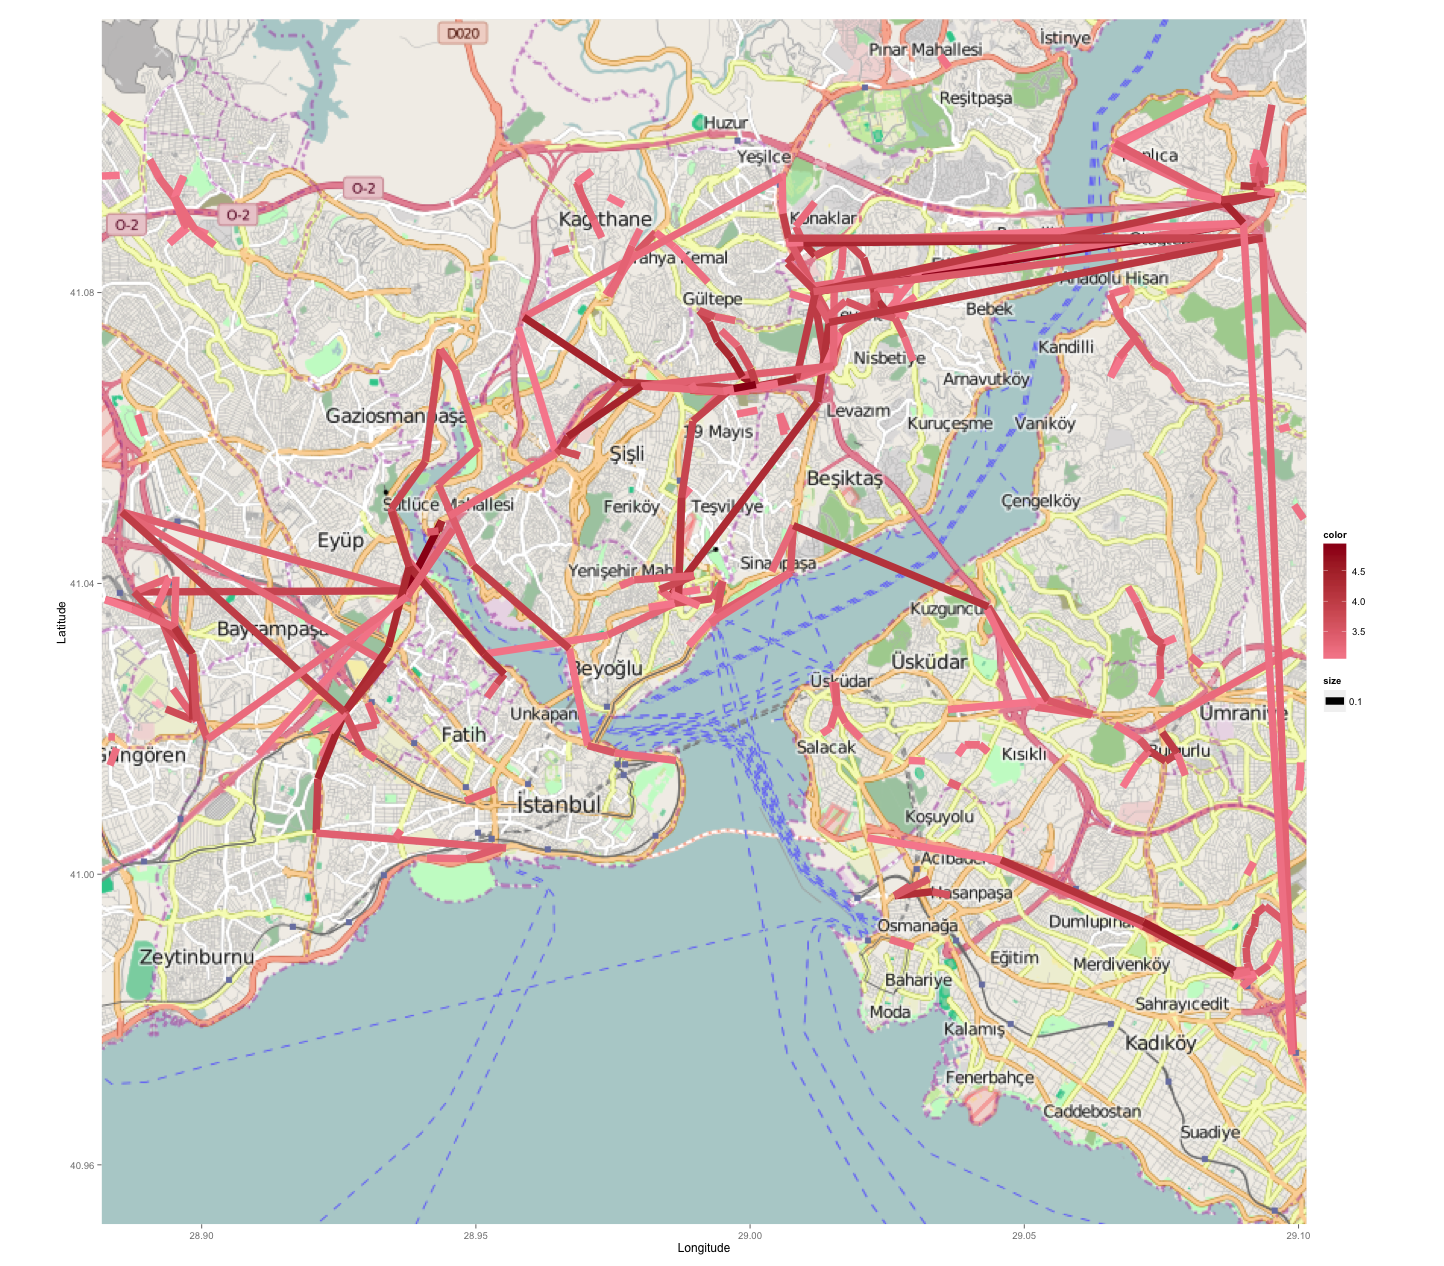
\includegraphics[width=0.94\linewidth]{img/map3-edge-betweenness.png}
  \caption{\textbf{Logaritmik Kenar Arasındalığı Haritası}. Koyu
   renkteki kenarların kenar arasındalık değeri daha yüksektir.}
  \label{fig:edgebetweenness}
\end{subfigure}
\begin{subfigure}{.5\textwidth}
  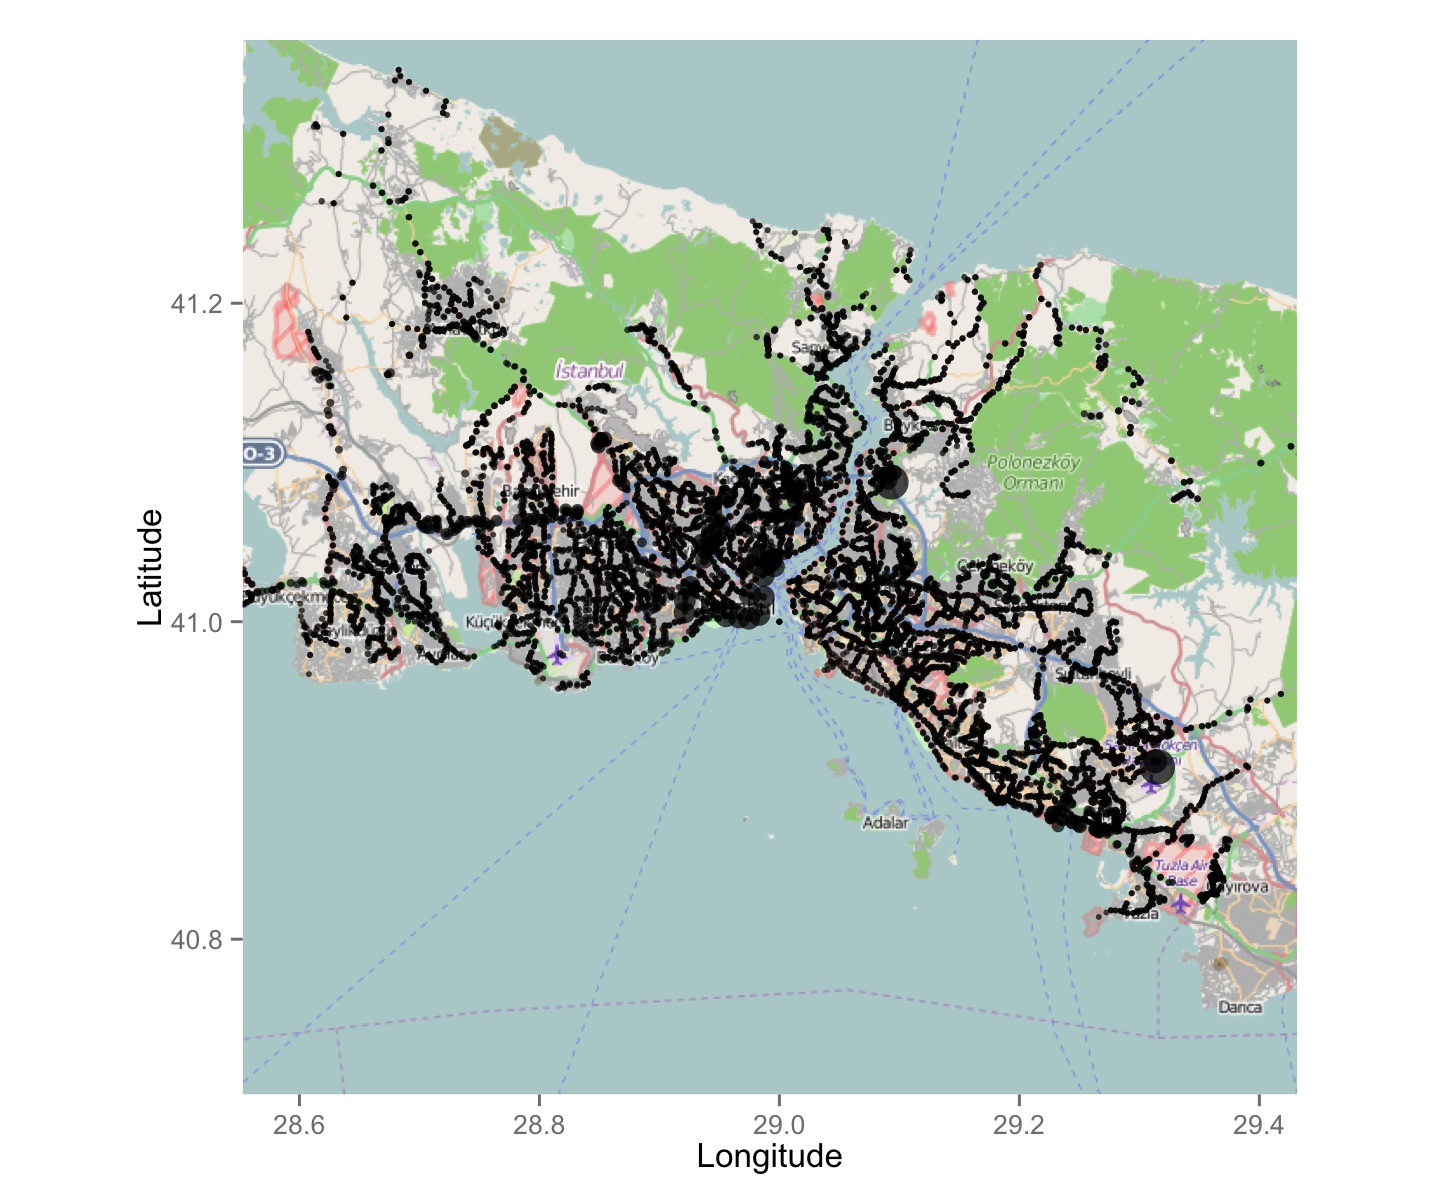
\includegraphics[width=\linewidth]{img/map4-node-betweenness.png}
  \caption{\textbf{Logaritmik Düğüm Arasındalığı Haritası}. Büyük ve koyu renkteki düğümlerin düğüm arasındalık değeri daha yüksektir.}
  \label{fig:node-betweenness}
\end{subfigure}
\caption{İstanbul toplu taşıma ağı görselleri}
\label{fig:fig}
\end{figure}

\end{document}